
%%% Local Variables:
%%% mode: latex
%%% TeX-master: t
%%% End:

\chapter{引言}
\label{cha:intro}

本章将介绍本文的相关背景,常用的凸包围体种类及应用,常见的碰撞检测算法及本文的结构安排。


\section{相关背景}

随着计算机软硬件技术的不断升级和发展,人们的衣食住行都越来越离不开计算机。
计算机图形学、计算机动画和虚拟现实等相关技术已经融入人类的日常生活当中,成为人们生活的重要组成部分,如医学领域的虚拟手术、设计领域的三维建模造型技术,日常生活中的电影游戏等等。

凸包围体技术在计算机图形学领域里的各种算法中发挥着重要作用,
如优化渲染和建模,加速求交、碰撞检测等。
以求交算法为例,如果两个模型相交,则对应的凸包围体一定相交,若凸包围体不相交则原始模型一定不相交。
凸包围体作为原始模型的近似,通常情况下,判断凸包围体是否相交比判断原始模型相交更简单,因此利用这个性质就可以加速模型之间的相交检测。
计算机图形学领域里常见的~AABB(Axis Aligned Bounding Box)包围盒和计算几何领域里的凸包都是凸包围体。
凸包围体有多种应用,主要是利用其“凸”的性质和可用来近似被包含模型的特征,应用于模型化简、碰撞检测等。
在几何计算过程中,包围体也用于相交等操作中进行预判和剪枝以提升整体算法的运行效率。

碰撞检测问题是计算机图形学、虚拟现实等领域中的研究热点,是计算机模拟真实环境中不可或缺的技术,在物理仿真及游戏领域里应用广泛。
例如在游戏中,碰撞检测技术增强了游戏的真实性,游戏中的角色行走不可穿墙、角色中弹而亡等等都离不开碰撞检测技术。

下面将分别介绍凸包围体相关技术和碰撞检测相关算法。

\section{凸包围体}
\label{sec:convex-bv}

对于“凸”定义如下(以二维欧式空间为例):
给定点集$S = \{p_1, ..., p_n\} \subseteq E^2$,如果有
$\lambda = (\lambda_1,...,\lambda_n)^T \in R^n, \lambda_1 + ... + \lambda_n = 1
$~且~ $min\{\lambda_1,...\lambda_n\} \geq 0$,我们称点 $p = [p_1, ... ,
p_n]\lambda = \lambda_1 p_1 + ... + \lambda_n
p_n$~为~$S$~的一个凸组合。一个点集~$P \subseteq E^2$~为凸的集合,当且尽当~$P$~的子集的凸组合仍然是$P$的子集。
更形象地讲,如果一个二维欧式空间的多边形是凸的,那么连接任意多边形内的两点构成的线段仍然在这个多边形的内部。

凸包围体能用于在原始模型之间的相关计算(遮挡测试、相交测试等)之前进行预处理判断和裁剪的理论基础正是基于此。通常来讲(无特别强调,本文不考虑包围体比原始模型还复杂的情况),凸包围体之间的计算比包含的原始模型计算更简单,当凸包围体之间没有相交或遮挡时,原始模型一定没有相交或遮挡。

根据具体的应用场景的不同有不同形状的凸包围体,常见的如下。

\subsection{AABB 包围体}

AABB(Asix Aligned Bounding Box)包围体是最常见最简单的包围体,俗称包围盒,其方向始终沿着坐标轴方向\cite{bergen1997efficient}。
在平面中就是包含二维模型的矩形,如图\ref{fig:aabb-bunny}所示,为平面图形~Bunny~的~AABB~包围体(二维情况称包围矩形更合适,但为了统一,这里统称包围体,后同)。对应到三维空间中就是沿坐标轴方向包含模型的最小的长方体。

\begin{figure}[htbp] % use float package If you want it here
  \centering
  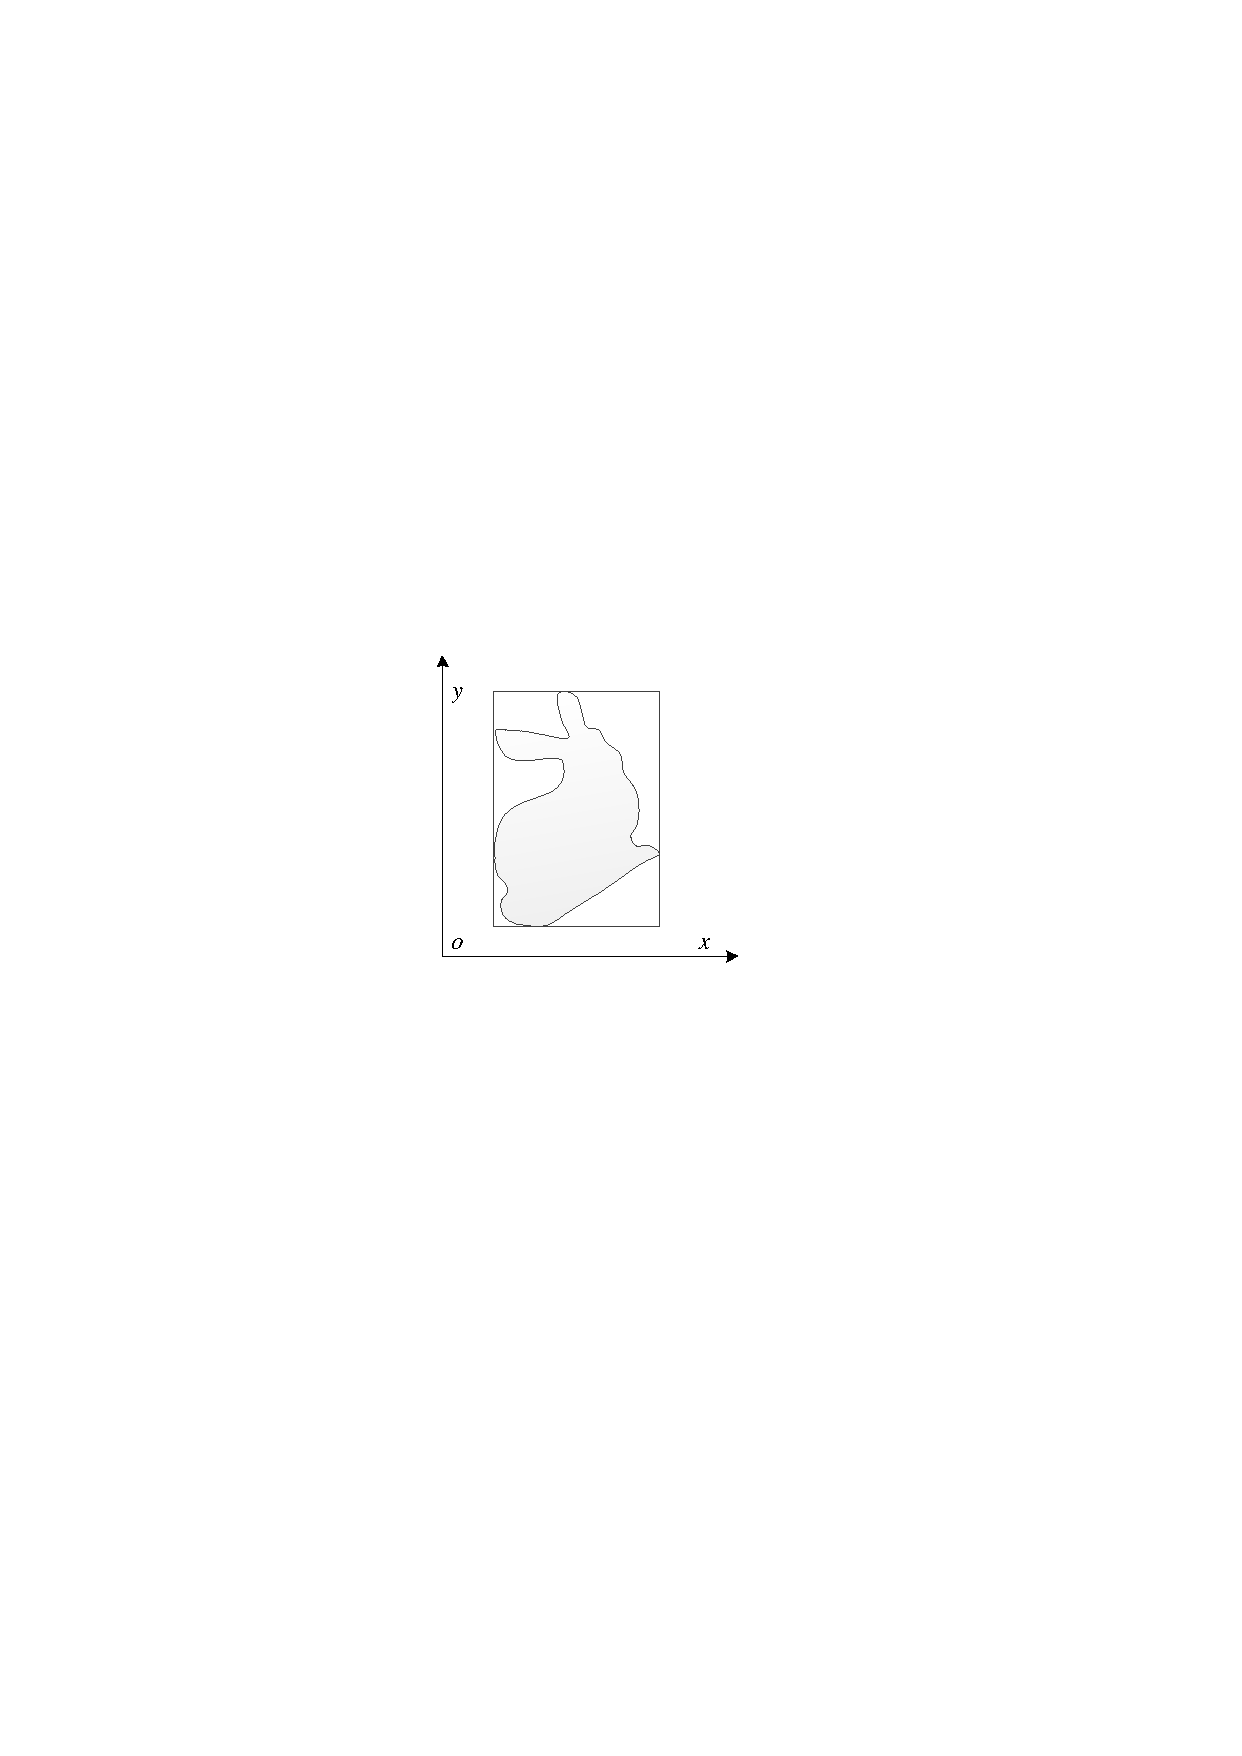
\includegraphics[width=1.5in]{bunny-2d-AABB.pdf}
  \caption{AABB 包围体}
  \label{fig:aabb-bunny}
\end{figure}

AABB~包围体的数据结构通常有3种方式:
\begin{inparaenum}[(1)]
\item 存储~AABB~包围体对角线上的两个极点,$Point_{min}$和$Point_{max}$,著名的计算几何库~CGAL\footnote{CGAL, Computational Geometry Algorithms Library, http://www.cgal.org}以此种方式存储;
\item 存储~AABB~包围体的中心点和各个方向的半径,$Point_{center}$和$Vector_{radius}$,如~SOLID\cite{bergen1997efficient};
\item 存储~AABB~包围体的极小点和各个方向的延伸长度\cite{ericson2005real},$Point_{min}$和$Vector_{extent}$。
\end{inparaenum} 

一方面~AABB~包围体之间的相交测试较简单,以数据结构为存储两个极点为例,只需要比较各个坐标值之间的大小即可。
但另一方面,通常情况下与原始模型的近似性较差,因其包围体的边沿着坐标轴方向可能会留较多的空白空间。

\subsection{OBB 包围体}

~OBB(Oriented Bounding Box)包围体是带方向的包围盒,可看作是~AABB~包围体沿任意方向转动一定角度后构成的包围体,因此通常情况下,~OBB~较~AABB~而言可以更紧致地贴近原始模型。
如图\ref{fig:obb-bunny}所示为平面图形~Bunny~的~OBB~包围体。

\begin{figure}[htbp] % use float package If you want it here
  \centering
  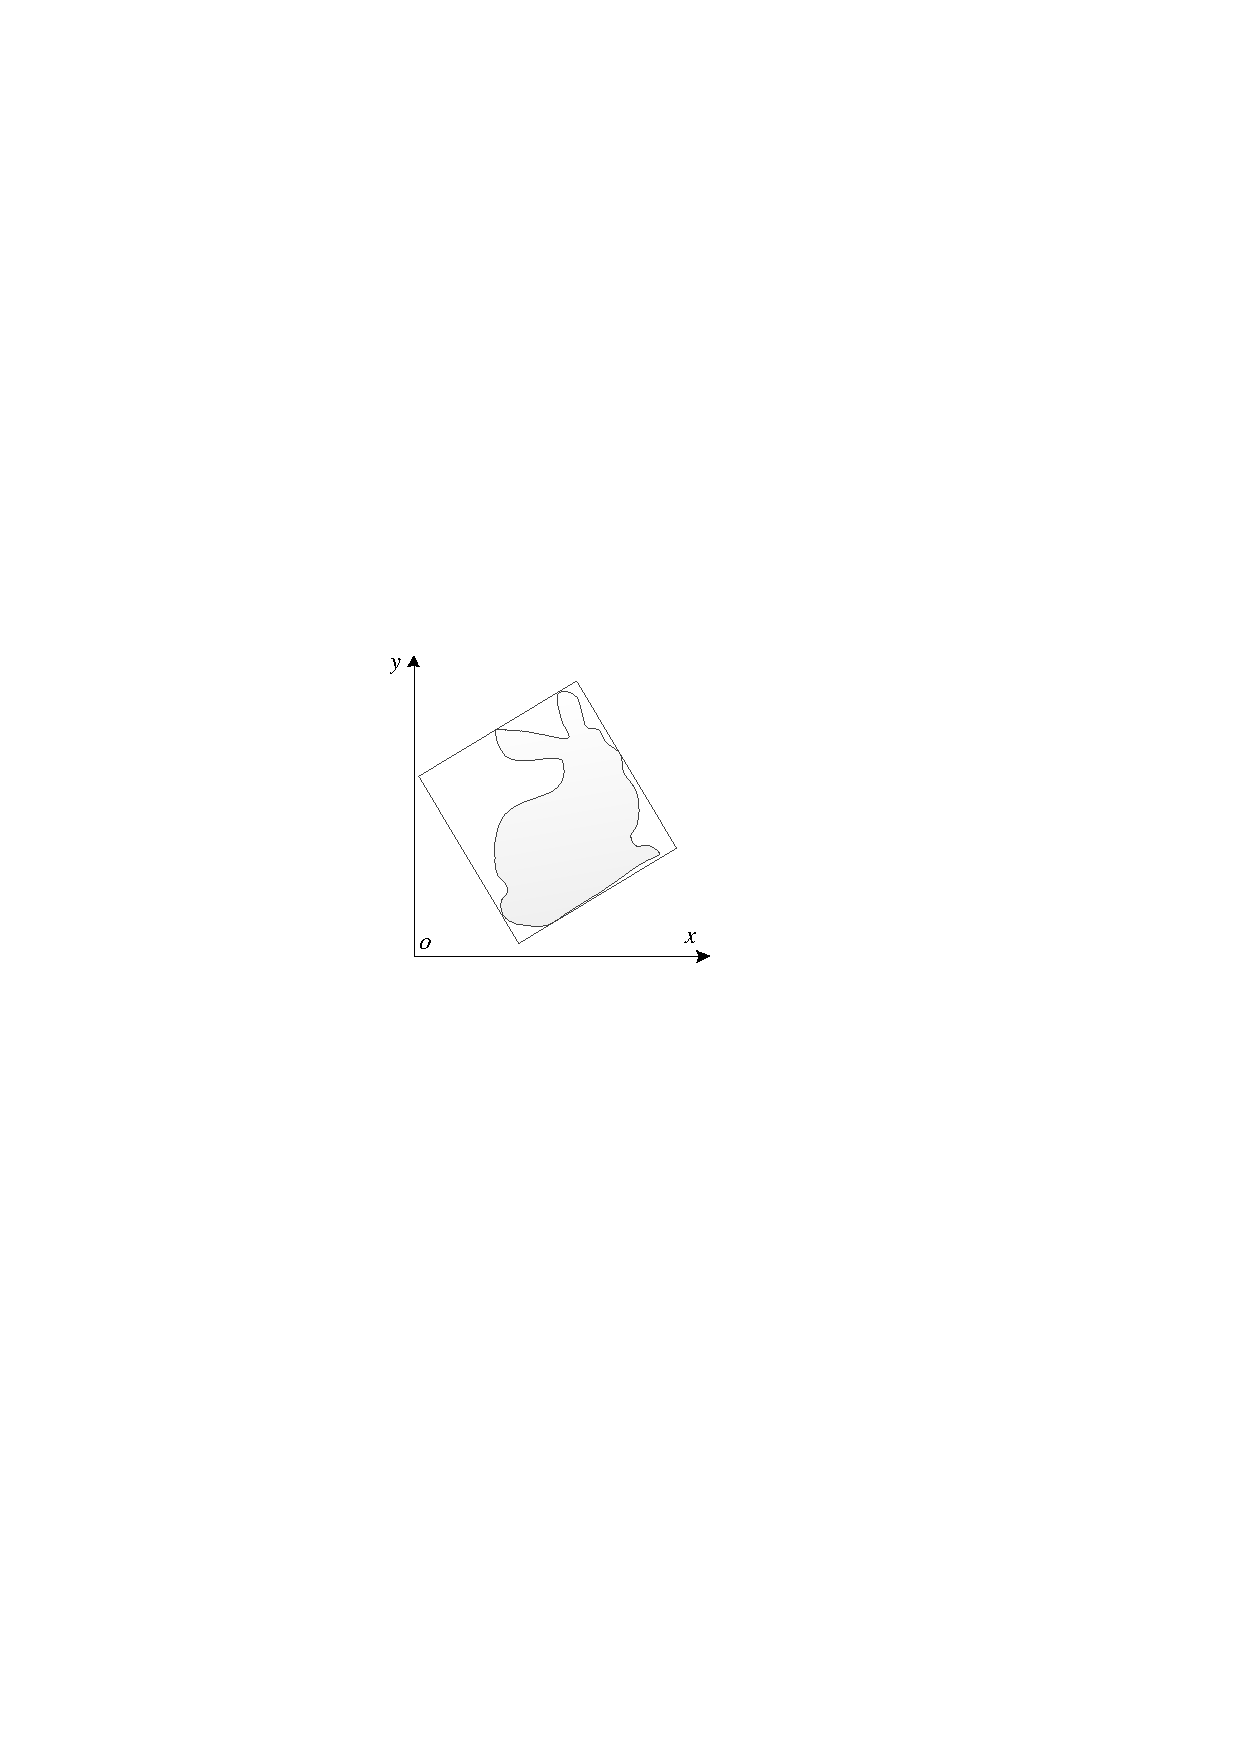
\includegraphics[width=1.5in]{bunny-2d-OBB.pdf}
  \caption{OBB 包围体}
  \label{fig:obb-bunny}
\end{figure}

与~AABB~类似,OBB~包围体的数据存储方式也可以有多种,最常用的是存储中心点,局部坐标架以及各个方向上的半径\cite{gottschalk1996obbtree}。因为~OBB~包围体的方向是任意的,有不少学者研究如何得到更加紧致的~OBB。

最早可追溯到由~O'Rourke~\cite{o1985finding}提出的$O(n^3)$
算法,文献\onlinecite{barequet2001efficiently}中提出了一种方法理论上可以在$O(n
+ 1/ \epsilon ^{4.5} )$复杂度内计算出一个近似最小~OBB($\epsilon$
为近似误差,即得到的$V\leq(1+\epsilon)\times V_{min}$,
其中$V$表示~OBB~的体积,$V_{min}$为最小~OBB~的体积),实际应用中通常实现的算法复杂度为$O(nlogn + n/
\epsilon ^{3} )$。~C.K.Chan~ \cite{chan2001determination}
提出了另外一种迭代的算法可以计算出误差范围内最小的~OBB~包围体,该算法适用于点数量较多(超过1万个点)的模型。

与~AABB~相比,~OBB~之间的相交测试稍复杂,需将二者转换到同一坐标系下进行计算,但其能更好的逼近原始模型。

\subsection{Sphere 包围体}

球形(Sphere)包围体,也称包围球(二维情况下即为包围圆,下同),即用一个半径尽量小的球包住给定所有点,该问题的求解是计算几何中的经典问题最小包围球的变种。
如图\ref{fig:sphere-bunny}所示为平面图形~Bunny~的~Sphere~包围体。

\begin{figure}[htbp] % use float package If you want it here
  \centering
  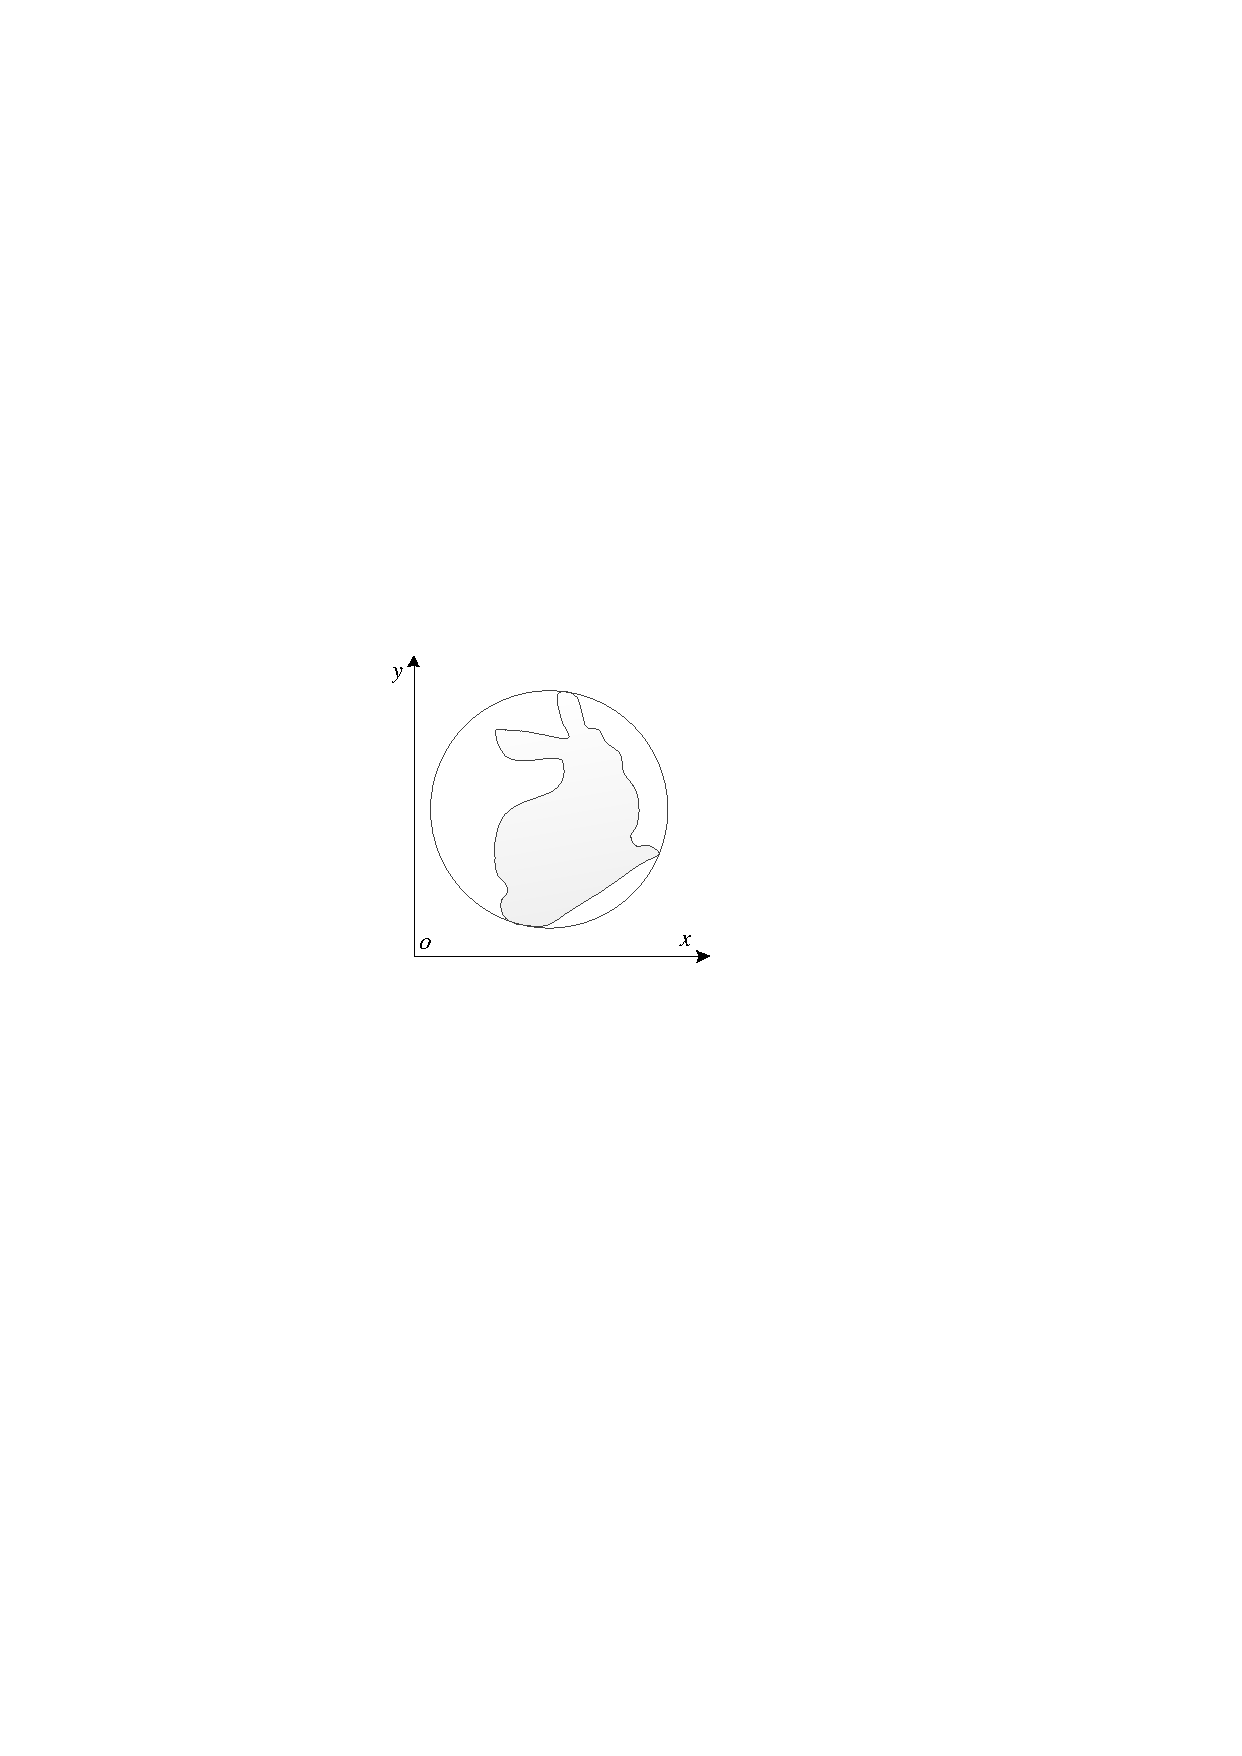
\includegraphics[width=1.5in]{bunny-2d-Sphere.pdf}
  \caption{Sphere 包围体}
  \label{fig:sphere-bunny}
\end{figure}

包围球的数据结构较简单,只需要球心和半径。一种最简单的计算一个包围求的方法是将相应~AABB~包围体的中心点作为球心,半径是为~AABB~各方向半径的最大值,这种方法虽然计算较快,但得到的包围体往往不够紧致。为了得到最小包围球,~E.Welzl~\cite{Welzl1991Smallest}
提出了一种线性的随机算法求出最小包围球。~T.Larsson~\cite{larsson2008fast}提出了一种快速简单的算法,该算法基于选择$k$个极点生成$k/2$个方向构造包围球,因而称为~EPOS~(Extremal Points Optimal Sphere~)算法,可以自定义$k$ 的值,能够给执行时间和包围盒紧致性之间进行调整折衷,提高了灵活性。

测试两个包围球是否相交较简单,只需判断两个球心之间的距离是否大于两个球半径之和即可。

\subsection{$k$-DOP 包围体}

$k$-DOP(Discrete Orientation Polytope)包围体是一个由$k$个固定方向的半平面相交构成的凸多面体,其最早思想来源于~TL.Kay~\cite{Kay1986Ray}
等人提出的用于解决光线追踪的问题,~$k$-DOP~术语是由~J.Klosowski~等人\cite{klosowski1998efficient}
在1998 年用于解决碰撞检测问题时提出的,有学者也称~$k$-DOP~为$k$-FDH($k$-Fixed
Directions Hull)\cite{weiyingmei2001}。
在二维(三维)平面上,~k-DOP~就是一个由$k/2$对平行的固定方向的边(面)围成的凸多边形(多面体),其中$k\in\mathbb{N}$,$k\geq4$($k\geq6$)。如图\ref{fig:8dop-bunny}所示,为平面图形~Bunny~的$8$-DOP。

\begin{figure}[htbp] % use float package If you want it here
  \centering
  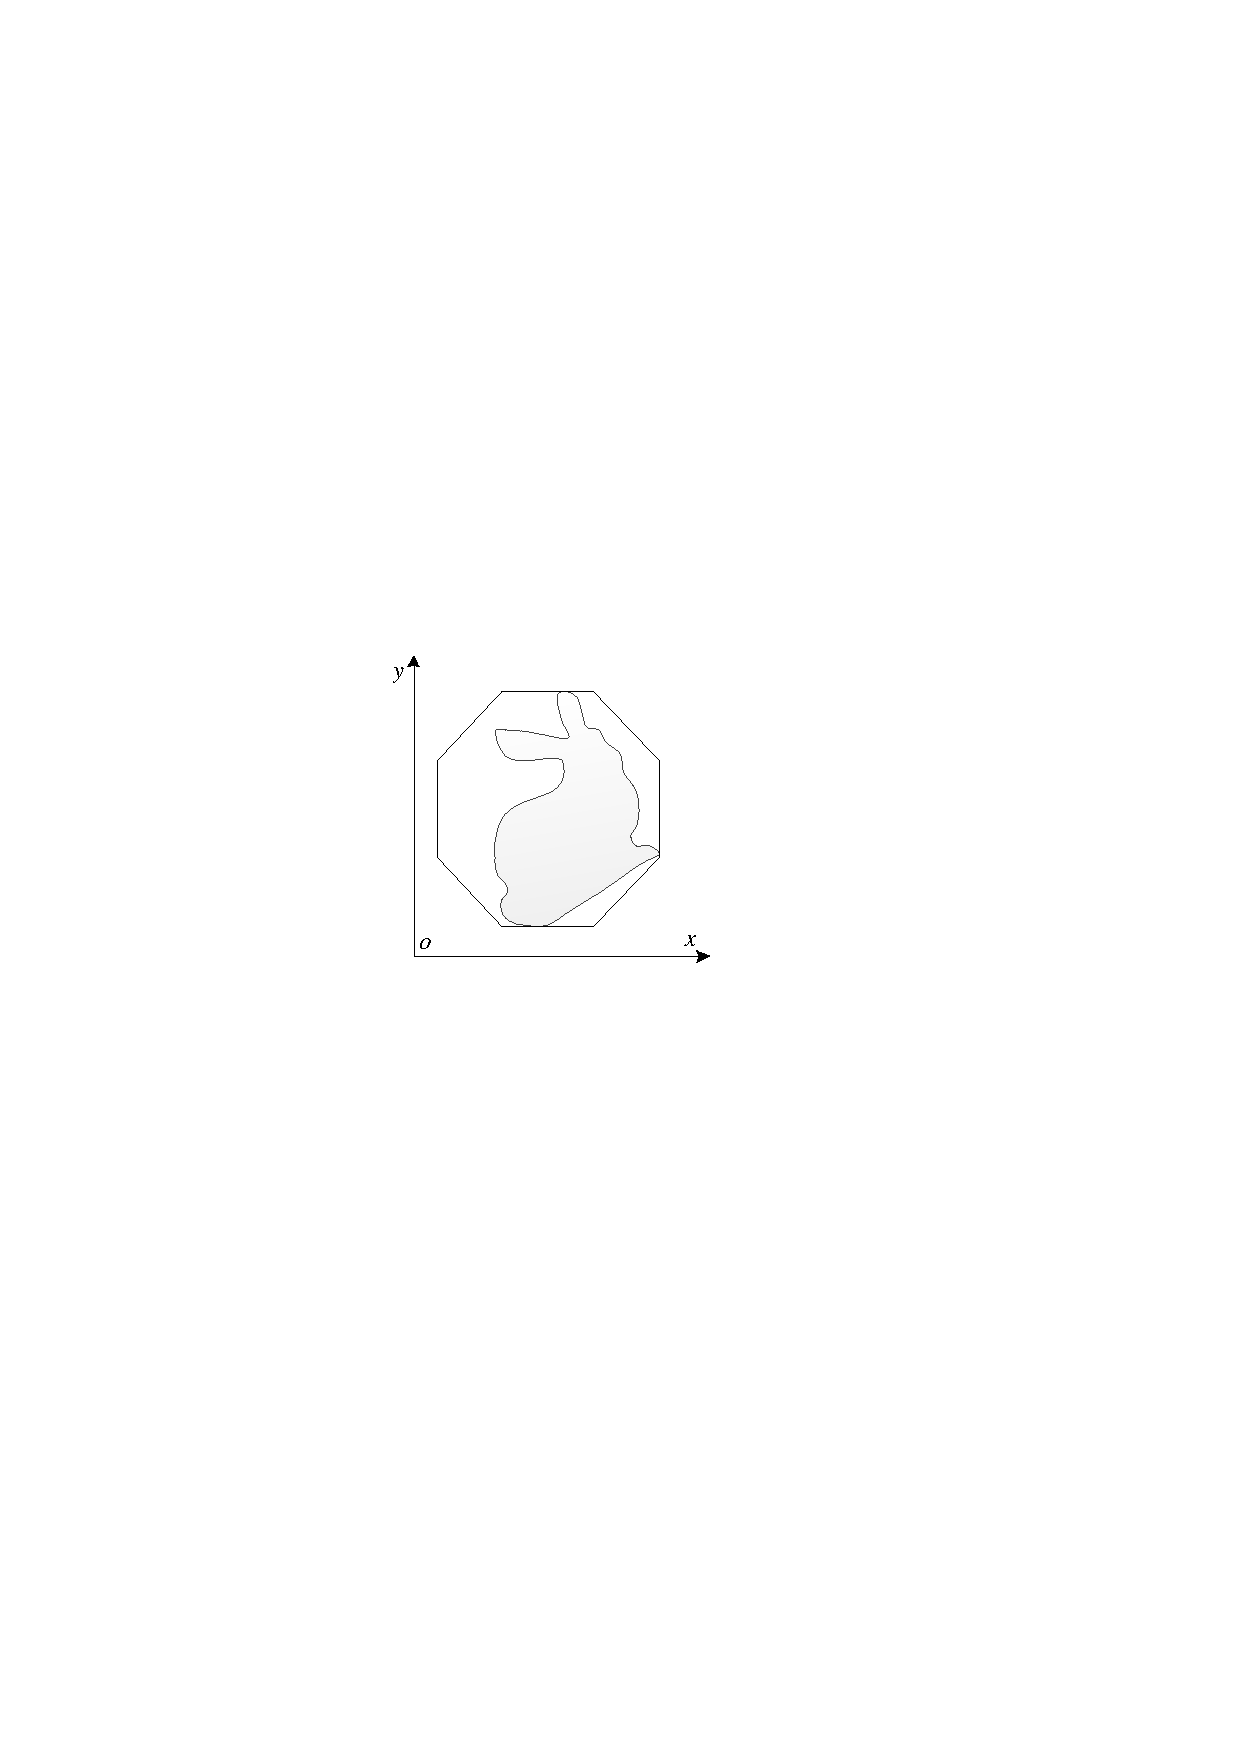
\includegraphics[width=1.5in]{bunny-2d-8DOP.pdf}
  \caption{$k$-DOP 包围体($k=8$)}
  \label{fig:8dop-bunny}
\end{figure}

对于$k$-DOP~中的每一个方向,可以由相应边(面)的法向决定,其数据结构一般用$k/2$个半平面的法向,再加上模型在各个方向上的投影的极值即可。因为$k$-DOP~的方向固定,$k$值确定后,相应的法向也随即确定,所以只需要存储各个方向的极值即可。当$k$-DOP~用于碰撞检测或可视化时,一般还需存储包围体的各个顶点。

~$k$-DOP~之间的相交测试将采用如算法~\ref{algo:kdop:overlaptest}~进行,即针对平行于~$k/2$~的每个方向去检测是否在指定的区间内。

\begin{algorithm}
\caption{$k$-DOP~相交测试算法}
\small
\label{algo:kdop:overlaptest}
\begin{algorithmic}[1]
\Require
$dop_1, dop_2, k$ 
\Ensure
两个~$k$-DOP~是否相交
\Function {CheckIntersection}{$dop_1, dop_2, k$}
  \For {$i = 0 \to k/2$}
      \If {$dop_1.min[i] >  dop_2.max[i] \textbf{~or~} dop_1.max[i] < dop_2.min[i]$}
          \State \Return \textbf{False} 
      \EndIf
  \EndFor
  \State \Return \textbf{True} \Comment{所有的区间都有重叠,$k$-DOP~一定相交}
\EndFunction
\end{algorithmic}
\end{algorithm}

与其他几种包围盒相比较而言,$k$-DOP~是取包围体存储计算和相交测试耗费时间的一个折衷,且可以通过修改$k$的值来提高包围体的灵活性。在不同的碰撞检测环境中可能选择不同的~$k$~值能达到更优的结果,
文献~\onlinecite{klosowski1998efficient}~中综合对比了~$k \in \{6,14,18,26\}$~,得出~$k=18$~时能达到效率最好的结果,而文献~\onlinecite{zachmann1998rapid}~经过实验发现在~$k \in \{6,8,14\}$~中,$k=6$~时能达到更好的结果,
事实上对于不同的碰撞检测测试环境,不同的模型而言,达到最优的结果选取的~$k$~值可能不都相同,文献~\onlinecite{abenchmarking2007}~在综合测试比较后有得出~$k=24$~时更容易得到更优的结果。


\subsection{Convex hull 包围体}
\label{subsec:convexhull}

凸包(Convex hull)是在计算几何中出现的概念,被定义为包含点集模型的最小凸集\cite{dengcg},
因此~Convex hull~包围体是最紧致的凸包围体,能够更好地近似模型本身。
包围体的紧致程度以凸包为衡量标准,一个包围体的紧致性 $\tau$ 按照如下公式计算:

\begin{equation}
\label{equa:judge:tightness}
\tau = \frac{V(CH)}{V(BV)}
\end{equation}

其中,$V(CH)$为凸包的体积,$V(BV)$~为包围体的体积,按照此公式计算出来的$\tau$越接近1表明其越紧致,凸包最紧致,其紧致性值1。

图\ref{fig:convexhull-bunny}为二维凸包的示例。

\begin{figure}[htbp] % use float package If you want it here
  \centering
  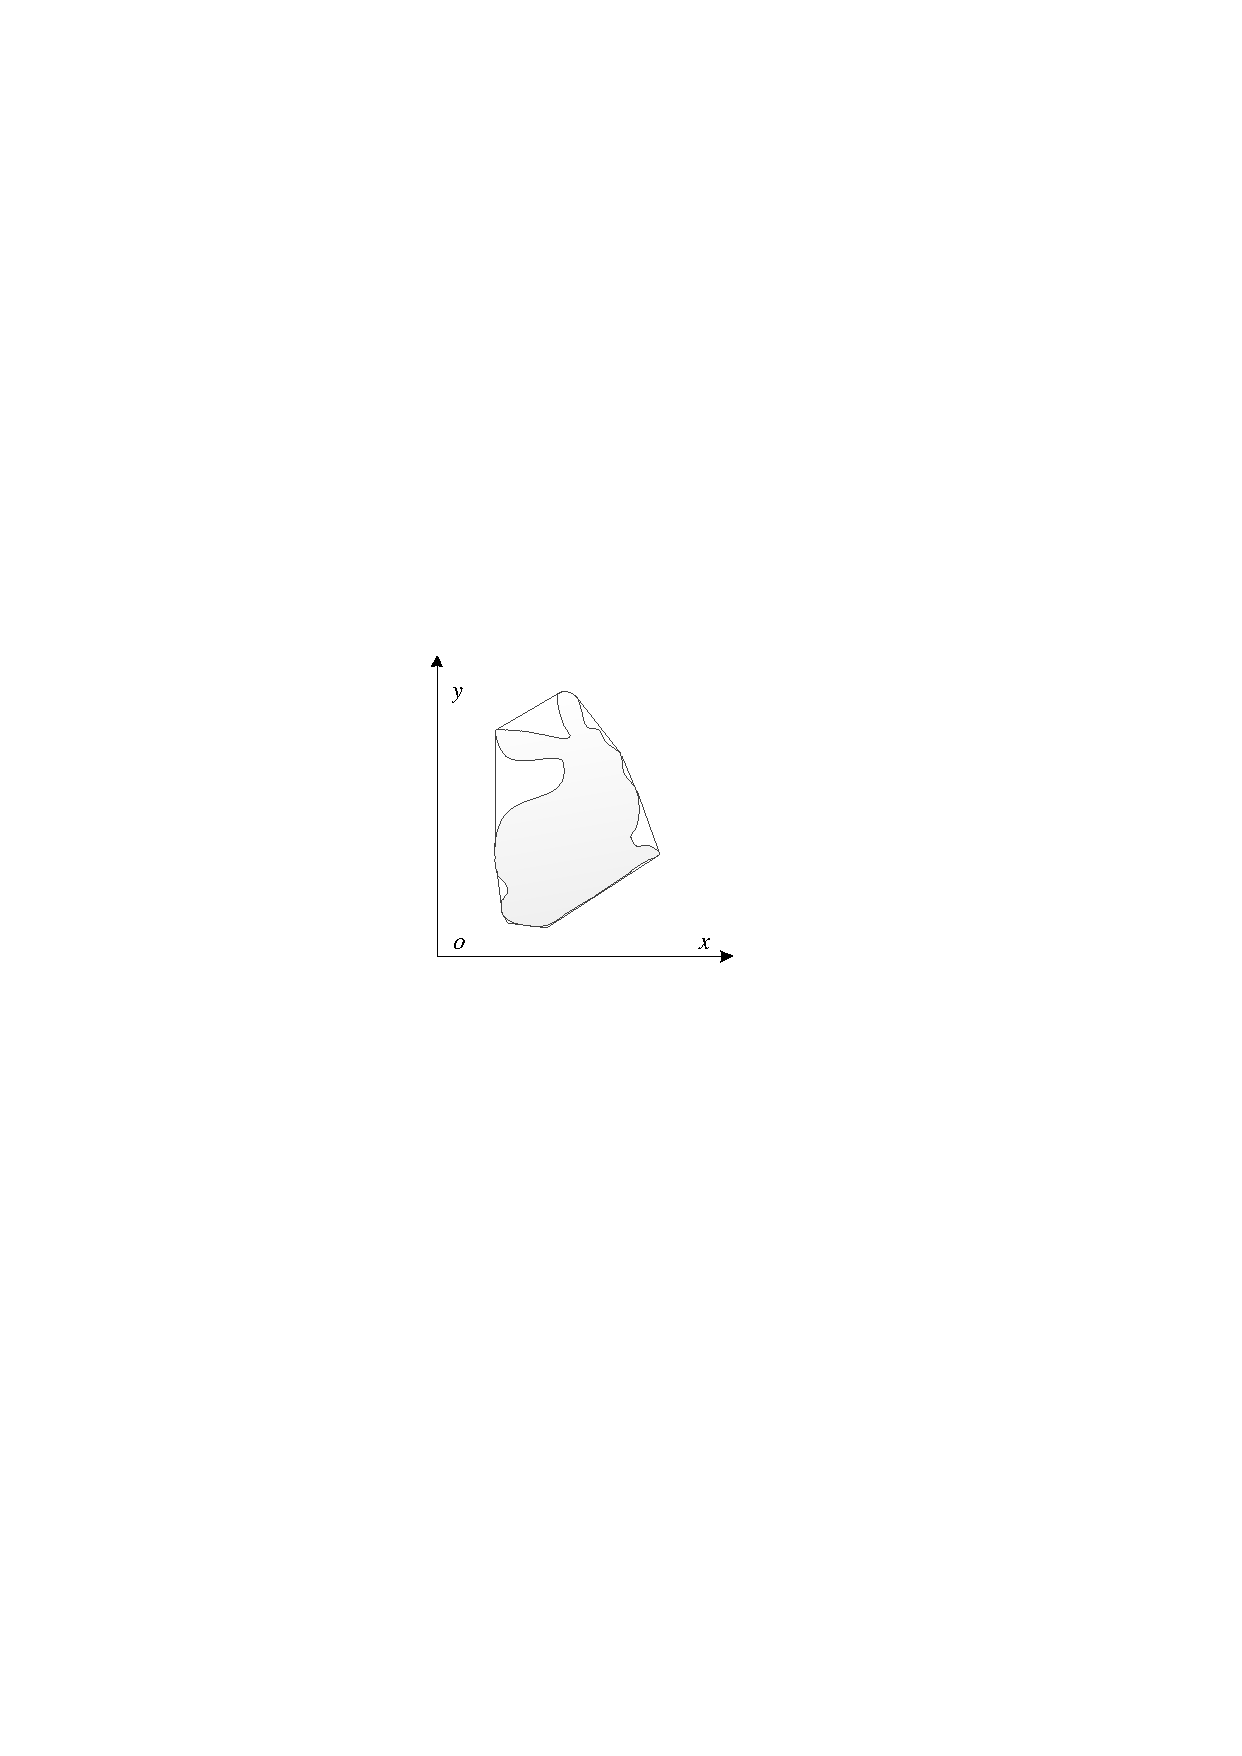
\includegraphics[width=1.5in]{bunny-2d-Convexhull.pdf}
  \caption{Convex hull 包围体}
  \label{fig:convexhull-bunny}
\end{figure}

常用的凸包构造算法有~Gift Wrapping~\cite{Chand1970An},复杂度最坏情况下为$O(n^2)$,构造凸包的算法时间复杂度下限为$O(n\log n)$,如~Preparata~提出的分治算法\cite{Preparata1977}。
当模型点集较大时,包围体涉及到的面片数量太多,做相交测试等相关计算时耗费时间较久,同时也耗费较多存储空间。因此~Convex hull~包围体不太适用于大模型。
为此有学者在一些应用中用到近似凸包,
近似凸包可分为三类:近似外凸包、近似内凸包和近似凸包\cite{hossain2013constructing},近似内凸包完全在精确凸包内部,近似外凸包完全包含精确凸包,近似凸包即与精确凸包有相交的地方。
文献\onlinecite{bentley1982approximation,kavan2006fast}介绍了两种计算近似内凸包的算法,文
献\onlinecite{Zunie1992}介绍了一种计算二维近似外凸包算法,本文算法在生成法向时就借鉴了文献\onlinecite{bentley1982approximation}中的近似凸包算法。

\subsection{其他包围体}

除了以上几种常见的凸包围体外,不同学者在特定领域里也研究出以下另外几种包围体:\\
\begin{inparaenum}[(1)]
\indent
\item \textbf{Tribox} 可以看作是$k$-DOP~的一种特例,其中,二维中$k=8$ ,三维中$k=18$。 文献\onlinecite{crosnier1999tribox} 中提出的方法可以方便构造~Tribox~层次结构,并应用于模型分解中,当投影方向固定时,对于运动对象,更新其~Tribox~包围体也比较方便。 \\ 
\indent
\item \textbf{Swept-sphere}
是由~Eric.Larsen~等人\cite{Larsen1999Fast}提出的一种用于查询两个物体之间准确和近似相隔距离的解决方案,因而也用于碰撞检测的应用当中,该包围体有多种变种。原文中给出了球沿直线做拉伸构成的~Line-swept-sphere(如图\ref{fig:subfig-bv-swept-sphere}所示)
以及沿矩形拉伸构成的~Rectangle-swept-sphere~等阐述,并提出了构造层次结构包围体的算法,还对哪些包围体合适做碰撞检测,哪些包围体合适做最近距离计算做了分析和说明,更多内容可以参考文献\onlinecite{Larsen1999Fast}。\\
\indent
\item \textbf{Sphere-shell}
文献\onlinecite{krishnan1997spherical}给出了一种“球壳”(Sphere-shell)包围体,该包围体由两个同球心不同半径的球中间围成的壳与锥点为球心的锥面相交部分构成,如图\ref{fig:subfig-spherical-shell}所示。这种球壳包围体有利于非结构化的模型、多边形集合(Polygon
soups~)模型之间(如简单多边形,样条曲面构成的模型)的相隔距离计算或者进行碰撞检测。\\
\indent
\item \textbf{Zonotopes} 2003 年,~Leonidas
J.Guibas~\cite{Guibas2003Zonotopes}等人利用对偶的方法提出了一种用线段表示三维包围盒的隐式表达法,称其为~Zonotopes(二维称为~Zonogon),这种方法不用显示描述记录构成包围盒的多面体的每个面,节省存储,而同样能够在较快的时间内进行碰撞检测等。\\
\indent
\item \textbf{其他}
还有如图\ref{fig:subfig-bv-cylinder}所示的圆柱形\cite{Schomer2000Smallest}、图\ref{fig:subfig-bvcone}所示的圆锥形\cite{held1997erit}和如图\ref{fig:subfig-bv-ellipse}所示的椭球形\cite{Wang2004Efficient}等等包围体。
\end{inparaenum}

\begin{figure}[htbp]
  \centering%
  \subcaptionbox{圆柱形包围体\label{fig:subfig-bv-cylinder}}%[3cm] %标题的长度
    {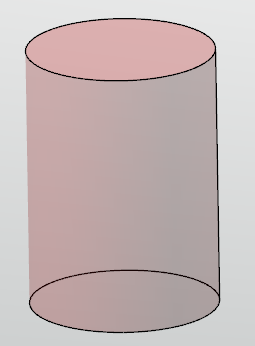
\includegraphics[height=4cm]{bv-cylinder.png}}
  \subcaptionbox{Sphere-shell~包围体\label{fig:subfig-spherical-shell}}
    {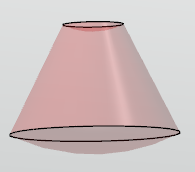
\includegraphics[height=4cm]{bv-spherical-shell.png}}
  \subcaptionbox{圆锥形包围体\label{fig:subfig-bvcone}}
    {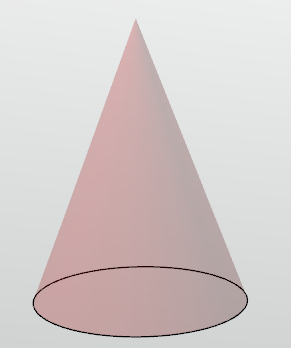
\includegraphics[height=4cm]{bv-cone.png}}
  \\
  \subcaptionbox{椭球形包围体\label{fig:subfig-bv-ellipse}}
    {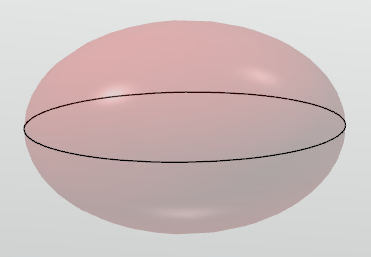
\includegraphics[height=4cm]{bv-ellipse.png}}
  \subcaptionbox{Swept-sphere~包围体\label{fig:subfig-bv-swept-sphere}}
    {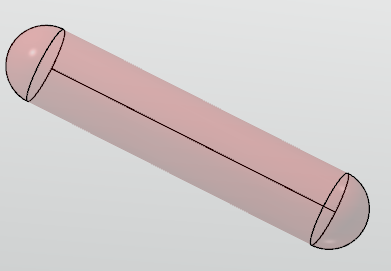
\includegraphics[height=4cm]{bv-swept-sphere.png}}
  \caption{其他包围体}
  \label{fig:bv-others}
\end{figure}

\subsection{包围体的应用}

包围体常见的应用领域有真实感渲染如可见面判别、视域剔除\cite{assarsson2000optimized},光线追踪\cite{wald2007ray}等。
在光线追踪算法中,包围体用于检测光线是否与物体相交,如果光线没有与包围体相交,则肯定不会与包围体内的物体模型相交,进而就不用渲染显示该物体。
另外更常见的应用就是碰撞检测\cite{wangzhiqiang1999},大多数碰撞检测算法都用到了各式各样的包围体以加速,如
\onlinecite{larsson2006dynamic,madera2009hybrid,vogiannou2010enhancing,chang2010efficient,tang2010fast,zhigang2010efficient} 等。

有不少文献将包围体和模型简化技术结合起来,例如~Kai Huebner~等人\cite{huebner2008minimum}在利用文献
\onlinecite{barequet2001efficiently}中提出的构造最小~OBB~包围体算法的基础上将物体分解成多个~OBB~包围体,用这些~OBB~包围体近似原始模型用于机器人抓取中,如图\ref{lbl:Huebner2008-example}所示。
类似的还有~Sphere~包围体的分解\cite{hubbard1996approximating}(如图\ref{lbl:hubbard1996approximating-example}),~Tribox~的分解\cite{crosnier1999tribox}等。

\begin{figure}[htbp]
  \centering
  \subcaptionbox{模型简化成~OBB~包围体\cite{huebner2008minimum}\label{lbl:Huebner2008-example}}%[3cm] %标题的长度
    {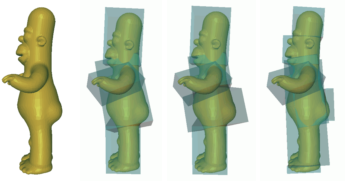
\includegraphics[height=4cm]{Huebner2008-example.png}}
  \subcaptionbox{模型简化成~Sphere~包围体\cite{hubbard1996approximating}\label{lbl:hubbard1996approximating-example}}
    {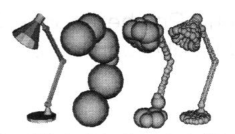
\includegraphics[height=4cm]{hubbard1996approximating-example.png}}
  \caption{包围体应用于模型简化}
  \label{lbl:bounding-voluems-used-in-shape-approximation}
\end{figure}

Jyh-Ming Lien~\cite{lien2006approximate2d}等人在06年提出一种方法可以将给定的多边形(包括含有孔洞的)分解成多个凸多边形,并提供不同种精度的分解,可以应用于~LoD(Level of
Detail,多层次细节)~,并在07年将其扩展到三维\cite{lien2007approximate3d},即提出了一种方法将原始实体模型近似为层次结构的凸包围多面体,如图\ref{lbl:lien2007approximate-example}
所示,对图中的原始模型进行准确凸分解(~ECD,Exact Convex
Decompositions~)将得到726240个组成部分,而近似凸分解(~ACD,Approximate Convex
Decompositions~)仅得到98个组成部分,同时保持了原始模型的大致形状,这大大加速了渲染过程。

\begin{figure}[htbp]
\centering
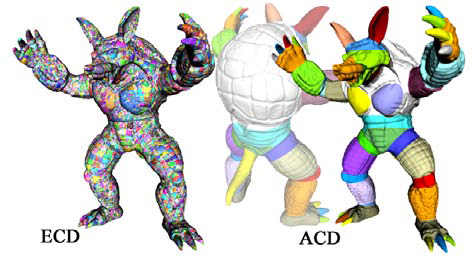
\includegraphics[width=3in]{lien2007approximate-example.png}
\caption{层次结构凸包围多面体的精确构造和近似构造\cite{lien2007approximate3d}}
\label{lbl:lien2007approximate-example}
\end{figure}
这种分解还可以应用于多种应用,例如运动规划(~Motion planning~),网格生成(~Mesh generation~),点定位(~Point location~)问题等等,更多内容可以参考\cite{lien2008approximate} 以及~Jyh-Ming Lien~ 的博士学位论文\cite{lien2006approximatephd}。

文献\cite{attene2008hierarchical}利用一种类似的方法将原始3D模型分解成一个具有层次结构的模型(图\ref{lbl:attene2008hierarchical-example:subfig1}所示),最顶层将是整个模型的凸包。将该算法应用到3D编辑环境中,能够更加方便地让用户选择模型的某个部分进行交互设计。效果如图\ref{lbl:attene2008hierarchical-example:subfig2} 所示,用户选择模型的头部,并进行拖拽能够较快速得到模型新的外观。\footnote{详情可参考视频:http://www.readcube.com/articles/10.1111/j.1467-8659.2008.01271.x }

\begin{figure}[htbp]
  \centering
  \subcaptionbox{层次结构的分解\label{lbl:attene2008hierarchical-example:subfig1}}
    {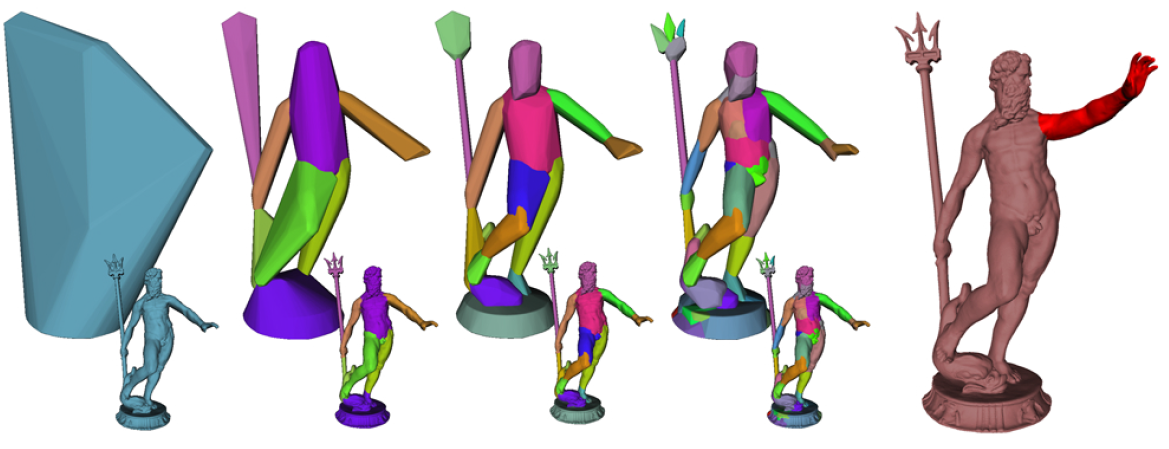
\includegraphics[height=2.8cm]{attene2008hierarchical-example-0.png}}
  \subcaptionbox{区域选择进行交互设计 \label{lbl:attene2008hierarchical-example:subfig2}}
    {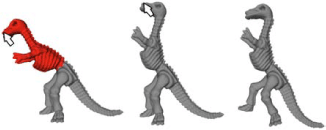
\includegraphics[height=2.8cm]{attene2008hierarchical-example.png}}
  \caption{层次结构的凸包围体及其应用于交互设计\cite{attene2008hierarchical}}
  \label{lbl:attene2008hierarchical-example}
\end{figure}

随着计算机软件技术和硬件的发展,有不少并行算法来计算包围体。
文献\cite{karlsson2010parallel}利用~Intel~单指令多数据流(Single Instruction
Multiple Data~,简称SIMD)~SSE~指令集和~OpenMP~实现了对~AABB~,~OBB~和~$k$-DOP~的计算。
文献\cite{lauterbach2009fast}提出了在~统一计算设备架构(Compute UnIfied Device
Architecture,简称CUDA,后同)~平台上基于~GPU~构造~AABB~包围体树的方法并应用于光线追踪。

\section{碰撞检测算法}
\label{sec:collisiondetection}

碰撞检测是许多应用的基础,例如在~3D~游戏,物理仿真,机器人,虚拟现实等。本节将就碰撞检测问题的分类和基于包围体树的算法进行阐述。

\subsection{碰撞检测算法的分类}
\label{sec:cd-category}

碰撞检测算法按照不同的分类标准可以有不同的分类方法。
根据其利用的加速结构不同大致可以分为两类,
一类是空间划分树(Spatial Partition Tree~,四叉树,八叉树,~KD~
树等),如文献\onlinecite{Melax2000}就提出了一种基于~BSP~的算法应用于~3D~游戏中的碰撞检测。
另外一种就是层次结构包围体(Bounding Volume Hierarchies
,简称~BVH,也称包围体树),如在\ref{sec:convex-bv}提到的~AABB~,~OBB~等包围体树。
包围体树跟常见的空间划分树最大的区别就是,在~BVH~中的两个或多个包围体可以包含相同的空间,而空间划分树的每个划分结构是分离的,且在~BVH~中,父节点不一定必须完整包含子节点,只需要包含子节点对应原始物体的那部分即可\cite{ericson2005real}。 
根据参与碰撞检测的物体模型的表现形式,又可以分为凸体模型或凹体模型,多边形或者三角网格模型,CSG~(Constructive
Solid Geometry,构造实体几何)模型,隐式方程或者参数表达曲面模型等,例如文献\onlinecite{Zeiller1995}就讨论了计算机动画系统中基于CSG模型的碰撞检测算法,GJK(Gilbet Johnson Keerthi)~算法\cite{gilbert1988fast,bergen1999fast}
是用来计算凸体模型之间的距离,因而常用于针对凸体模型之间的碰撞检测算法。
根据碰撞检测的模拟环境划分,又可以分为成对(Pair Processing)碰撞检测和多体(Nbody Processing)碰撞检测,刚体和柔性模型的碰撞检测以及静态和动态(连续)碰撞检测\cite{lin1998collision}。
文献\onlinecite{jimenez20013d}从碰撞检测的解决策略上做了系统的分类和总结,文中提到目前的碰撞检测都是从几何或代数的方法进行求解,其中几何方法主要利用投影、采样或者二者的结合的技术进行处理。

随着~3D~扫描仪的出现,近年来也出现了一些基于点云的碰撞检测算法。Klein Jan~等人\cite{klein2004point}首次在~EuroGraphics 04~上提出了点云的碰撞检测概念,同样利用了层次结构包围体进行加速检测,并提出了一个给定容差的判断点云模型之间是否相交的算法。
文献\cite{figueiredo2010efficient}将~AABB~包围体和~R~树结合起来,并从~OAABB(Overlapped AABB)中找出是否含有一个模型的点在容差范围内逼近另外一个点云模型以此判断是否发生相交。

随着计算机图形卡的产生,又不断涌现出基于~GPU~的碰撞检测并行算法,如文献\onlinecite{Zhang2007Interactive,hebing2009}等,利用~GPU~多线程技术提高碰撞检测的效率。

\subsection{基于包围体树的碰撞检测算法}
\label{sec:cd-bvh}

在第\ref{sec:convex-bv}节中介绍了在对原始几何模型进行求交判断之前先用其包围体判断是否相交有助于提高求交过程的性能,
通过将包围体组织成树形结构即层次结构包围体(BVH)能够将包围体预判阶段从理论上降低到对数时间复杂度(要求树是平衡的)。
当构造原始复杂模型的包围体树时,复杂模型会被拆分成多个部分,每个部分用某种包围体近似,这构成了树型结构的叶子节点,这些节点会按照某种分组策略进行合并成更大的包围体分别构成其父节点,如此递归,最终形成一颗树,树最顶端是一个包含住原始物体的最粗糙的包围体,如图\ref{lbl:bvh-example}
所示,为一个8层~AABB~包围体的~BVH(也可以看作是8层6-DOP的~BVH)。
\begin{figure}[htbp]
  \centering
  \subcaptionbox*{\label{lbl:bvh-bunny-center-0.png}}
    {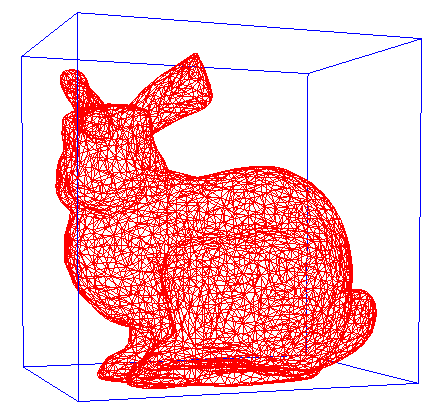
\includegraphics[height=2.8cm]{bvh-bunny-center-0.png}}
  \subcaptionbox*{\label{lbl:bvh-bunny-center-1.png}}
    {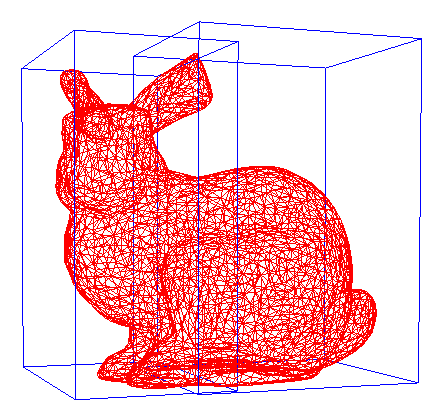
\includegraphics[height=2.8cm]{bvh-bunny-center-1.png}}
  \subcaptionbox*{\label{lbl:bvh-bunny-center-2.png}}
    {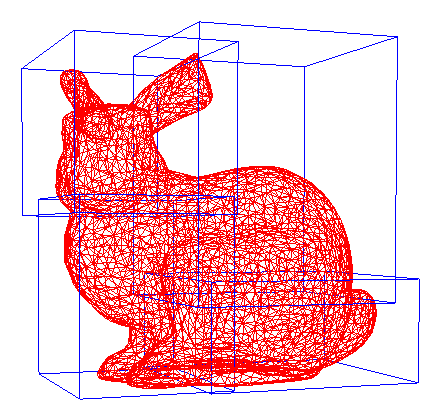
\includegraphics[height=2.8cm]{bvh-bunny-center-2.png}}
  \subcaptionbox*{\label{lbl:bvh-bunny-center-3.png}}
    {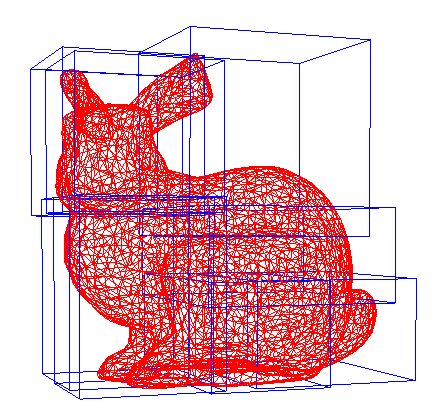
\includegraphics[height=2.8cm]{bvh-bunny-center-3.png}}
    \vspace{-0.3cm}
  \\\hspace{0.5cm} 
  \subcaptionbox*{\label{lbl:bvh-bunny-center-4.png}}
    {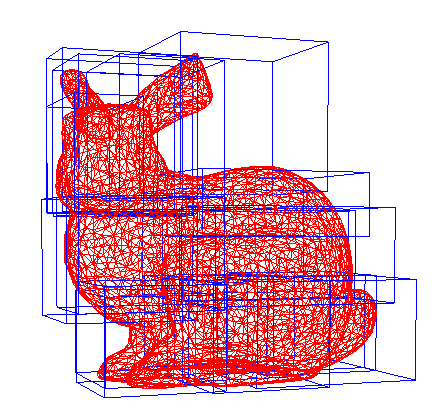
\includegraphics[height=3.0cm]{bvh-bunny-center-4.png}}
  \subcaptionbox*{\label{lbl:bvh-bunny-center-5.png}}
    {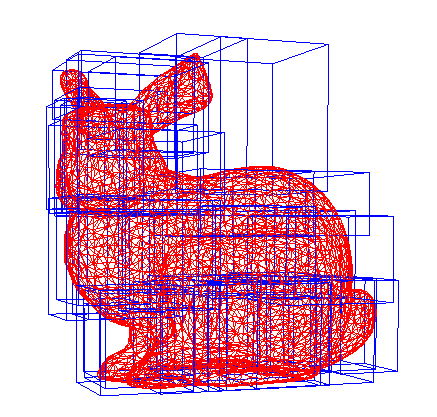
\includegraphics[height=3.0cm]{bvh-bunny-center-5.png}}
  \subcaptionbox*{\label{lbl:bvh-bunny-center-6.png}}
    {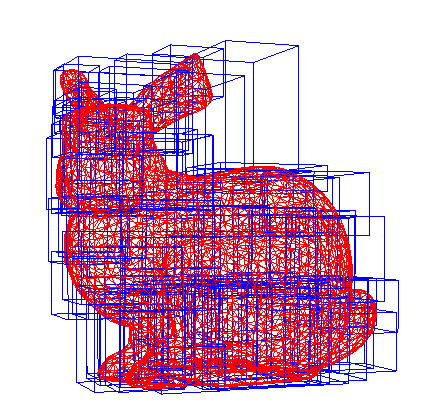
\includegraphics[height=3.0cm]{bvh-bunny-center-6.png}}
  \subcaptionbox*{\label{lbl:bvh-bunny-center-7.png}}
    {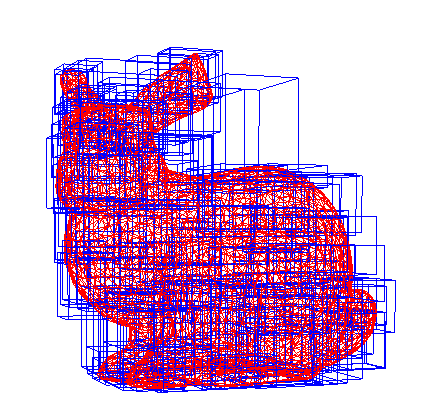
\includegraphics[height=3.0cm]{bvh-bunny-center-7.png}}
\caption{八层~BVH~示例}
\label{lbl:bvh-example}
\end{figure}

在碰撞检测算法中,一般会对模型进行预处理建立起各自的~BVH~树,当两个模型进行相交检测时,自顶向下遍历两棵~BVH~树,若父节点没有相交,则没有必要进行子节点的相交测试,自顶向下的层次遍历算法如算法~\ref{alg:traverse-bvh-tree}~所示。

\begin{algorithm}
%\algsetup{linenosize=\tiny}
\small
\caption{自顶向下层次遍历~BVH~}
\label{alg:traverse-bvh-tree}
\begin{algorithmic}[1]
\Require
$node_1$,$node_2$:BVH~树中的节点1、节点2
\Ensure
是否相交
\Function {TraverseBVHTree}{$node_1, node_2$}
  \If{$node_1.bv \cap node_2.bv = \emptyset$} 
    \State \Return{\textbf{False}} 
    \Comment{包围体重合测试, 包围体不相交直接返回}
  \Else
      \If {$node_1.children = \emptyset$}
           \If {$node_2.children = \emptyset$}
              \State {$\Return \Call{CheckIntersection}{node_1.primitives, node_2.primitives}$} \Comment{最底层叶子节点原生几何相交测试}
           \Else
              \ForAll {$child \in node_2.children$}
              \State \Call{TraverseBVHTree}{$node_1, child$} \Comment{递归调用}
              \EndFor
           \EndIf
      \Else
           \ForAll {$child \in node_1.children$}
           \State \Call{TraverseBVHTree}{$child, node_2$}  \Comment{递归调用}
           \EndFor
      \EndIf
  \EndIf
\EndFunction
\end{algorithmic}
\end{algorithm}

从算法~\ref{alg:traverse-bvh-tree}~可以看出,基于~BVH~的碰撞检测算法性能的好坏关键在于两个操作,一是分别来自两个~BVH~内部节点包围体之间的相交测试,二是~BVH~最底层叶子节点内的原生几何相交测试,
常常利用公式~\ref{equa:evaluate:static:bv}~来衡量单个相交测试的所付出的代价
\begin{equation}
T_{cost} = n_v * C_v + n_p * C_p,
\label{equa:evaluate:static:bv}
\end{equation}
其中$n_v$
和$n_p$分别表示参与包围体节点相交测试的数量和参与原始几何相交测试的数量,$C_v$和$C_p$则表示相应的平均测试耗费的代价\cite{klosowski1998efficient}。
当运动场景或连续碰撞的模型之间的碰撞检测时,往往还需要考虑到因物体模型旋转平移等变换产生的包围体的更新所付出的代价,即上述代价函数变成
\begin{equation}
T_{cost} = n_v * C_v + n_p * C_p + n_u * C_u
  \label{equa:evaluate:dynamic:bv}
\end{equation}
其中~$n_u$~和~$C_n$~就是模型旋转或者运动后包围体更新的数量和更新的代价。要提高碰撞检测的性能,就得想办法减小$T_{cost}$的值。
%本文的算法主要关注于静态场景。

不同的包围体,上述代价函数各个值不同,对于不同的应用场景,可能需要选择不同的包围体进行加速碰撞检测。
文献\onlinecite{zhigang2010efficient}从包围体的构造难度,包围体的紧致性,包围体之间相交测试复杂性及包围体在运动过程中的更新代价几个方面对五种常见的包围体进行了比较,如表\ref{lbl:table:bv-comp}所示。
可以看出,各种包围体有各自的优缺点和适用场景,因此,很多研究人员充分利用各种包围体的优点,将多种包围体结合在一起组成新的组合包围体。
文献\cite{chang2010efficient}利用~OBB~包围体相对的紧致优点和球形包围体相交测试简单性的优点进行组合,构造~OBB-Sphere~包围体,在进行相交测试时,先利用球形包围体进行测试,如果相交再用~OBB~进行测试。
类似的,文献\cite{zhigang2010efficient}同时利用更加紧致的$k$-DOP~和~Sphere~包围体构造$k$-DOP-Sphere~包围体。

\begin{table}[htbp]
\centering
\caption{碰撞检测中常用凸包围体比较}
\begin{tabular}{ccccc}
\toprule[1.5pt]
凸包围体 & 构造代价 & 相交测试简单性 & 紧致性 & 更新代价\\
\midrule[1.0pt]
AABB   & 1 & 2 & 4 & 3\\
OBB    & 4 & 4 & 3 & 2\\
Sphere & 2 & 1 & 5 & 1\\
k-DOP  & 3 & 3 & 2 & 4\\
Convex hull & 5 & 5 & 1 & 5 \\
\bottomrule[1.5pt]
\end{tabular}
\label{lbl:table:bv-comp}
\end{table}


\section{本文主要内容}
\label{sec:structure}
本文着重讨论如何快速地生成紧致性可控的凸包围体以及将此包围体应用于静态场景的碰撞检测。
第一章首先介绍了当前各种凸包围体的特征及应用。然后再介绍了碰撞检测问题的背景和本文研究的基于凸包围体的碰撞检测算法。

第二章提出了紧致性可控的凸包围体$k$-CBP($k$-Convex Bounding Polyhedron)~的生成算法,紧致性可控主要通过凸包围体的平面数量$k$来调节。
该算法法首先利用近似内凸包和~$k$-means~聚类算法生成构成凸包围多面体~$k$~个截面的法向,
然后根据输入点集沿各法向搜索切点构成截面,最后由这些截面通过对偶映射的方式求交构成凸包围多面体。
在搜索截面过程中,提出了两种并行策略以加速搜索过程。实验结果表明,与同类算法相比,该方法能够更快地构造给定点集更紧致的凸包围多面体。

第三章提出了基于本文提出的$k$-CBP~包围体的碰撞检测算法,在包围体之间的相交测试时分别用~AABB~树的方式和基于~GJK~算法的两种方式进行。
实验结果表明本文提出的凸包围体能够有效加速碰撞检测算法。

第四章是对本文的研究工作进行总结,以及未来可以改进的方向。
